\documentclass[tikz,dvipsnames]{standalone}
\usetikzlibrary{backgrounds}
\usetikzlibrary{calc}
\usetikzlibrary{arrows.meta}
\usetikzlibrary{positioning}

\begin{document}
 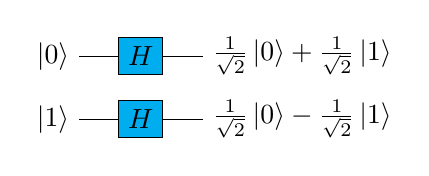
\begin{tikzpicture}[
    show background rectangle,
    tight background=0,
    background rectangle/.style={fill=white},
    node distance=0.5,
 ]
    \node (X0) {$|0\rangle$};
    \node[right=of X0,draw, fill=cyan] (H0) {$H$};
    \node[right=of H0] (Y0) {$\frac{1}{\sqrt{2}}\,|0\rangle+\frac{1}{\sqrt{2}}\,|1\rangle$};
    \draw (X0) -- (H0) -- (Y0);
    
    \node[below=0.2 of X0] (X1) {$|1\rangle$};
    \node[right=of X1,draw, fill=cyan] (H1) {$H$};
    \node[right=of H1] (Y1) {$\frac{1}{\sqrt{2}}\,|0\rangle-\frac{1}{\sqrt{2}}\,|1\rangle$};
    \draw (X1) -- (H1) -- (Y1);
\end{tikzpicture}
\end{document}
